\section{Experiments}\label{s:exp}

In this section we compare our method to several strong baselines.
We start by describing the datasets and the baselines, followed by a quantitative and a qualitative evaluation.


\newcommand{\rottext}[1]{\centering\rotatebox{90}{#1}}
\newcommand{\rotmpage}[1]{
\begin{minipage}[c][2cm][c]{0.1cm}%
% \begin{minipage}[c][\imh][c]{0.1cm}%
\rottext{#1}%
\end{minipage}%
}
\newcommand{\wcolone}{1.2cm}
\newcommand{\td}{TD}

\begin{table}[t]
\caption{%
\textbf{Monocular multi-hypothesis human mesh recovery} comparing our approach to
two multi-hypothesis baselines (SMPL-CVAE, SMPL-MDN) and
state-of-the-art single mode evaluation models \cite{kolotouros19learning,kolotouros19convolutional,kanazawa18end-to-end}
on Human3.6m (H36M), its ambiguous version AH36M, on 3DPW and its ambiguous version A3DPW.
}\label{tab:tab_quantitative}%
\vspace{0.2cm}
\centering \footnotesize
\begin{tabular}{c|c|cccccccc}
\toprule
\multirow{2}{\wcolone}{Dataset}      &
\multicolumn{1}{c}{Quantization $n$} & 
\multicolumn{2}{c}{1} & 
\multicolumn{2}{c}{5} & 
\multicolumn{2}{c}{10} & 
\multicolumn{2}{c}{25} \\ \cmidrule{2-10} 
& \multicolumn{1}{c}{Metric}
& MPJPE     & RE        
& MPJPE     & RE
& MPJPE      & RE        
& MPJPE      & RE        \\
\midrule
% ---------------------
% \multirow{6}{1cm}{\rotmpage{Human3.6m}}
\multirow{6}{\wcolone}{H36M}
& HMR~\cite{kanazawa18end-to-end}
& ---      & 56.8      
& ---       & ---       
& ---        & ---       
& ---        & ---       \\
& GraphCMR~\cite{kolotouros19convolutional}
& 71.9      & 50.1      
& ---       & ---       
& ---        & ---       
& ---        & ---       \\
& SPIN~\cite{kolotouros19learning}
& 62.2      & 41.8
& ---       & ---       
& ---        & ---       
& ---        & ---       \\
& SMPL-MDN                
& 64.4  & 44.8 
& 61.8  & 43.3       
& 61.3  & 43.0
& 61.1  & 42.7      \\
& SMPL-CVAE                
& 70.1  & 46.7      
& 68.9  & 46.4      
& 68.6  & 46.3      
& 68.1  & 46.2      \\
% & \multicolumn{1}{l}{\textbf{Ours}}
& \textbf{Ours}
& \textbf{61.5} & \textbf{41.6}
& \textbf{59.8} & \textbf{42.0}
& \textbf{59.2} & \textbf{42.2}
& \textbf{58.2} & \textbf{42.2}
\\
\midrule
\multirow{6}{\wcolone}{3DPW}
& HMR~\cite{kanazawa18end-to-end}
& ---   & 81.3      
& ---   & ---       
& ---   & ---       
& ---   & ---       \\
& GraphCMR~\cite{kolotouros19convolutional}
& ---   & 70.2      
& ---   & ---       
& ---   & ---       
& ---   & ---       \\
& SPIN~\cite{kolotouros19learning}
& 96.9  & \textbf{59.3}
& ---   & ---       
& ---   & ---       
& ---   & ---       \\
& SMPL-MDN                
& 105.8 & 64.7
& 96.9  & 61.2
& 95.9  & 60.7     
& 94.9  & 60.1     \\
& SMPL-CVAE                
& 96.3  & 61.4      
& 93.7  & 60.7      
& 92.9  & 60.5      
& 92.0  & 60.3      \\
& \textbf{Ours}
& \textbf{93.8} & 59.9
& \textbf{82.2} & \textbf{57.1}
& \textbf{79.4} & \textbf{56.6}
& \textbf{75.8} & \textbf{55.6}
\\ 
\midrule
\multirow{4}{\wcolone}{AH36M}
% & SPIN~\cite{kolotouros19learning}
% & \td  & \td      
% & ---   & ---       
% & ---   & ---       
% & ---   & ---       \\
& SMPL-MDN                
& 113.9  & 74.7
& 98.0   & 70.8
& 95.1   & 69.9     
& 91.5   & 69.5     \\
& SMPL-CVAE                
& 114.5  & 76.5
& 111.5  & 75.7     
& 110.6  & 75.4     
& 109.7  & 75.1     \\
& \textbf{Ours}
& \textbf{103.6} & \textbf{67.8}
& \textbf{96.4}  & \textbf{67.1}
& \textbf{93.5}  & \textbf{66.0} 
& \textbf{90.0}  & \textbf{64.2}     \\

\midrule
\multirow{4}{\wcolone}{A3DPW}
% & SPIN~\cite{kolotouros19learning}
% & \td  & \td      
% & ---   & ---       
% & ---   & ---       
% & ---   & ---       \\
& SMPL-MDN                
& 159.7  & 82.8
& 154.6  & 83.0
& 149.6  & 80.7     
& 122.1  & 76.6     \\
& SMPL-CVAE                
& 156.6  & 80.2
& 154.5  & 79.9     
& 153.9  & 79.8     
& 153.1  & 79.8     \\
& \textbf{Ours}
& \textbf{149.6} & \textbf{78.5}
& \textbf{125.6}  & \textbf{74.4}
& \textbf{116.7}  & \textbf{73.7} 
& \textbf{107.8}  & \textbf{72.1}     \\



\bottomrule
\end{tabular}
%\vspace{-0.25cm}
\end{table}





% % 3dpw std
% \begin{table}[t]
% \centering
% \begin{tabular}{@{}ccccccccc@{}}
% \toprule
% Num Modes                & \multicolumn{2}{c}{1} & \multicolumn{2}{c}{5} & \multicolumn{2}{c}{10} & \multicolumn{2}{c}{25} \\ 
% \midrule 
% & MPJPE & RE        
% & MPJPE & RE
% & MPJPE & RE        
% & MPJPE & RE        \\
% \midrule
% HMR~\cite{kanazawa18end-to-end}
% & ---   & 81.3      
% & ---   & ---       
% & ---   & ---       
% & ---   & ---       \\
% GraphCMR~\cite{kolotouros19convolutiona}
% & \td  & TODO      
% & ---   & ---       
% & ---   & ---       
% & ---   & ---       \\
% SPIN~\cite{kolotouros19learning}
% & 96.9  & 59.3      
% & ---   & ---       
% & ---   & ---       
% & ---   & ---       \\
% SMPL-MDN                
% & TODO  & TODO
% & TODO  & TODO     
% & TODO  & TODO     
% & TODO  & TODO     \\
% SMPL-CVAE                
% & 97.0  & 60.6      
% & 96.7  & 60.6      
% & 96.6  & 60.6      
% & 96.5  & 60.5      \\
% \multicolumn{1}{l}{Ours} 
% & \textbf{93.8} & \textbf{59.9}      
% & \textbf{82.7} & \textbf{57.5}     
% & \textbf{79.9} & \textbf{57.0}     
% & \textbf{76.2} & \textbf{56.0}
% \\ \bottomrule
% \end{tabular}
% \caption{\textbf{Monocular multi-hypothesis human mesh recovery on 3DPW} comparing our approach to state-of-the-art models (designed for single mode evaluation) and two multi-hypothesis baselines.}\label{tab:tab_base_3dpw_std}
% \end{table}


% % AAA H36m
% \begin{table}[]
% \centering
% \begin{tabular}{@{}ccccccccc@{}}
% \toprule
% Num Modes                & \multicolumn{2}{c}{1} & \multicolumn{2}{c}{5} & \multicolumn{2}{c}{10} & \multicolumn{2}{c}{25} \\ 
% \midrule 
% & MPJPE     & RE        
% & MPJPE     & RE
% & MPJPE      & RE        
% & MPJPE      & RE        \\
% \midrule
% SMPL-MDN                
% & TODO  & TODO
% & TODO  & TODO     
% & TODO  & TODO     
% & TODO  & TODO     \\
% SMPL-CVAE                
% & TODO  & TODO
% & TODO  & TODO     
% & TODO  & TODO     
% & TODO  & TODO     \\
% \multicolumn{1}{l}{\textbf{Ours}}
% & TODO  & TODO
% & TODO  & TODO     
% & TODO  & TODO     
% & TODO  & TODO     \\
% \bottomrule
% \end{tabular}
% \caption{\textbf{Monocular multi-hypothesis human mesh recovery on AH36m (\MPJPE)} comparing our approach to two multi-hypothesis baselines.}\label{tab:tab_base_h36m_amb}
% \end{table}


% % 3dpw ablation
% \begin{table}[]
% \centering
% \begin{tabular}{@{}ccccccccc@{}}
% \toprule
% Num Modes                & \multicolumn{2}{c}{1} & \multicolumn{2}{c}{5} & \multicolumn{2}{c}{10} & \multicolumn{2}{c}{25} \\ 
% \midrule 
% & MPJPE     & RE        
% & MPJPE     & RE
% & MPJPE      & RE        
% & MPJPE      & RE        \\
% \midrule
% % BOTTOM LEFT
% Ours w/o Mode Reproj, Flow Weight
% & \textbf{93.0}      & \textbf{59.5}
% & 86.4       & 57.9
% & 84.0        & 57.5
% & 79.0        & 56.3       \\
% % BOTTOM RIGHT
% Ours w/o Mode Reproj
% & \textbf{93.0}       & \textbf{59.5}
% & 84.1       & 57.0
% & 81.9        & 56.7 
% & 77.8        & 55.8       \\
% % TOP LEFT
% Ours w/o Flow Weight
% & 93.8      & 59.9
% & 82.7       & 57.5
% & 79.9        & 57.0
% & 76.2        & 55.9       \\
% % TOP RIGHT
% \textbf{Ours}
% & 93.8 & 59.9
% & \textbf{82.2} & \textbf{57.1}
% & \textbf{79.4} & \textbf{56.6}
% & \textbf{75.8} & \textbf{55.6}
% \\ \bottomrule
% \end{tabular}
% \caption{\textbf{Monocular multi-hypothesis human mesh recovery on 3DPW} comparing our approach to state-of-the-art models (designed for single mode evaluation) and two multi-hypothesis baselines.}\label{tab:tab_base_h36m_amb}
% \end{table}
% \begin{table}[t]
% \centering
% \begin{tabular}{@{}lrrrr@{}}
% \toprule
% \multicolumn{1}{l}{Num Modes} & 
% \multicolumn{1}{c}{1}         & 
% \multicolumn{1}{c}{3}         & 
% \multicolumn{1}{c}{5}         & 
% \multicolumn{1}{c}{25}        \\ \midrule
% \multicolumn{1}{r}{Ours w/o Mode Reproj.} & 76.4             & 74.1              & 73.5              & 72.8                     \\
% \multicolumn{1}{r}{Ours w/o Flow} & \textbf{75.4}    & 73.7              & 73.5              & 71.3                     \\
% \multicolumn{1}{r}{Ours}         & 75.5             & \textbf{71.9}     & \textbf{71.0}     & \textbf{68.7}            \\ \bottomrule
% \end{tabular}
% \caption{\label{tab:abl_unambi}\textbf{Ablation study on H36m} removing either the normalizing flow or the mode re-projection losses and reporting the change in performance.}
% \end{table}



% \multicolumn{4}{c|}{Active Losses $\mathcal{L}$} & 

\begin{table}[t]
\caption{\textbf{Ablation study on 3DPW} removing either the normalizing flow or the mode re-projection losses and reporting the change in performance.}\label{tab:tab_abl}
\vspace{0.2cm}
\centering \footnotesize
\begin{tabular}{@{}cc|ccccccc@{}}
\toprule
\multicolumn{2}{c}{Quantization $n$} & 
% \multicolumn{2}{c}{1} & 
\multicolumn{2}{c}{5} & 
\multicolumn{2}{c}{10} & 
\multicolumn{2}{c}{25} \\ 
\midrule 
Mode reproj. & Flow weight
% & MPJPE     & RE        
& MPJPE     & RE
& MPJPE      & RE 
& MPJPE      & RE \\
\midrule
% BOTTOM LEFT
& 
% & \textbf{93.0}      & \textbf{59.5}
& 86.4       & 57.9
& 84.0        & 57.5
& 79.0        & 56.3       \\
% BOTTOM RIGHT
& \checkmark
% Ours w/o Mode Reproj
% & \textbf{93.0} & \textbf{59.5}
& 84.1       & \textbf{57.0}
& 81.9        & 56.7 
& 77.8        & 55.8       \\
% TOP LEFT
\checkmark &
% Ours w/o Flow Weight
% & 93.8      & 59.9
& 82.7       & 57.5
& 79.9        & 57.0
& 76.2        & 55.9       \\
% TOP RIGHT
% \textbf{Ours} 
\checkmark & \checkmark
% & 93.8 & 59.9
& \textbf{82.2} & 57.1
& \textbf{79.4} & \textbf{56.6}
& \textbf{75.8} & \textbf{55.6}
\\ \bottomrule
\end{tabular}
%\vspace{-0.45cm}
\end{table}

\paragraph{Datasets and evaluation protocol.}

Our evaluation focuses on the Human3.6m (\textbf{H36M})~\cite{ionescu2013human3,IonescuSminchisescu11} 
and \textbf{3DPW} datasets \cite{vonmarcard2018recovering}.
H36M is one of the largest datasets of humans annotated with 3D pose using MoCap sensors.
\begin{wrapfigure}{r}{0.45\textwidth}
  \begin{center}
           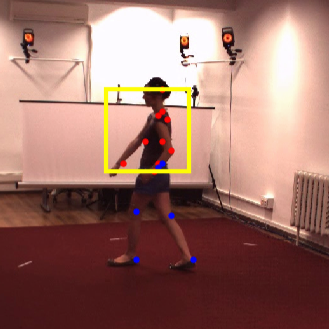
\includegraphics[width=0.49\linewidth]{exps/dataset_uncrop.png}
    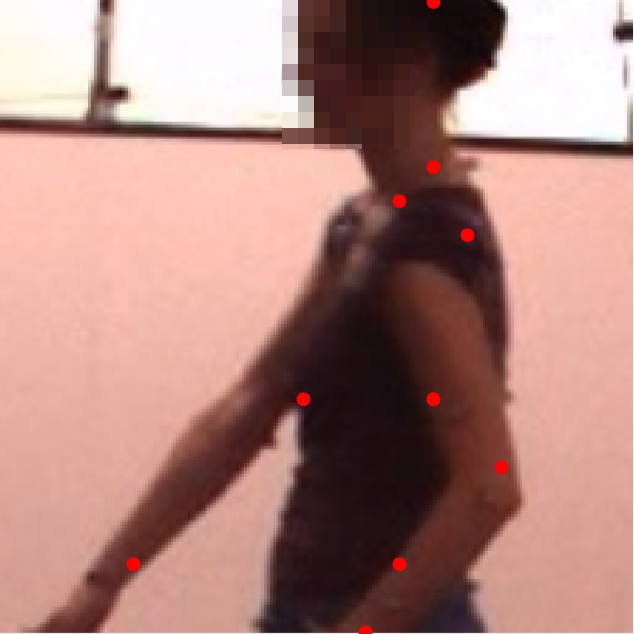
\includegraphics[width=0.49\linewidth]{exps/cropped3_blur.png}
  \end{center}
    \caption{Example image and corresponding annotation from the ambiguous H36M dataset \textbf{AH36M}. Best viewed in colour.\label{f:ambi_samples}}
    \vspace{-1.8em}
\end{wrapfigure}
As common practice, we train on subjects S1, S5, S6, S7 and S8, and test on S9 and S11. 3DPW is only used for evaluation and, following \cite{kolotouros19convolutional}, we evaluate on its test set.

Our evaluation is consistent with~\cite{kolotouros19learning,kolotouros19convolutional} - we report two metrics that compare the lifted dense 3D SMPL shape to the ground truth mesh: Mean Per Joint Position Error (\textbf{\MPJPE}), Reconstruction Error (\textbf{\RE}). 
For H36M, all errors are computed using an evaluation scheme known as ``Protocol \#2''. Please refer to supplementary for a detailed explanation of \MPJPE and \RE.

% We report three metrics that compare the lifted dense 3D SMPL shape to the ground truth mesh: Mean Per Joint Position Error (\textbf{\MPJPE}), Reconstruction Error (\textbf{\RE}), and dense Shape Error (\textbf{\SE}).
% All errors are computed using an evaluation scheme known as ``Protocol \#1'', as explained below.

% TODO: MOVE TO SUPPLEMENTARY
% For each H36M test skeleton, \MPJPE calculates the mean distance between 14 ground truth skeleton 3D joints and the predicted joints obtained by using a fixed linear regressor that maps the array of 6890 3D coordinates of the predicted dense mesh to the skeleton 3D joint coordinates.
% We report an average of all \MPJPE errors measured for each test skeleton.
% The reconstruction error is a modification of \MPJPE which consists of finding an additional rigid Procrustes alignment between the pair of assessed poses before evaluating the inter-joint distances.
% Finally, SE comprises a dense reconstruction metric that evaluates per-vertex distance error between each of the 6890 pairs of ground truth and predicted vertices of the evaluated SMPL meshes.

\paragraph{Multipose metrics.}

% \MPJPE, \RE and \SE 
\MPJPE and \RE are traditional metrics that assume a single correct ground truth prediction for a given 2D observation.
As mentioned above, such an assumption is rarely correct due to the inherent ambiguity of the monocular 3D shape estimation task.
We thus also report \MPJPE-$n$/\RE-$n$ an extension of \MPJPE\RE used in~\cite{li19generating}, that enables an evaluation of $n$ different shape hypotheses.
In more detail, to evaluate an algorithm, we allow it to output $n$ possible predictions and, out of this set, we select the one that minimizes the \MPJPE/\RE metric.
We report results for $n\in \{1,5,10,25\}$.

\paragraph{Ambiguous H36M/3DPW (AH36M/A3DPW).}
Since H36M is captured in a controlled environment, it rarely depicts challenging real-world scenarios such as body occlusions that are the main source of ambiguity in the single-view 3D shape estimation problem.

% Hence, in order to allow for a quantitative evaluation in a more noisy scenario, we construct an adapted version of H36M with synthetically-generated occlusions as follows 
Hence, we construct an adapted version of H36M with synthetically-generated occlusions (\cref{f:ambi_samples}) by randomly hiding a subset of the 2D keypoints and re-computing an image crop around the remaining visible joints. Please refer to the supplementary for details of the occlusion generation process.

While 3DPW does contain real scenes, for completeness, we also evaluate on a noisy, and thus more challenging version (A3DPW) generated according to the aforementioned strategy.

% We begin with the full size image with a set of 2D joints and apply synthetic occlusions to the subject's body parts by randomly hiding a subset of the 2D keypoints and re-computing a slightly padded image crop around the joints that remained visible. 
% For each image, we randomly choose one of 4 possible strategies for hiding the keypoints: 1) Hiding arm and head keypoints; 2) legs; 3) head; 4) no keypoints hidden\footnote{The selection probabilities are $p(1)=p(2)=p(3)=0.3$, $p(4)=0.1$}. 
% Please refer to the supplementary materials for details of the occlusion generation process.

% 3DPW contains real scenes, but for completeness, we also consider its noisy, and thus more challening, version (A3DPW) generated with the aforementioned strategy.

% \begin{figure}
% 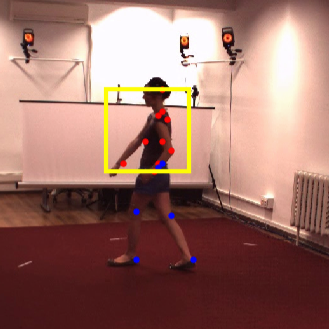
\includegraphics[width=0.49\linewidth]{exps/dataset_uncrop.png}
% \includegraphics[width=0.49\linewidth]{exps/cropped3.png}
% % \centering\fbox{\makebox(230,100){}}
% \end{figure}


\paragraph{Baselines}\label{s:exp_baselines}

Our method is compared to two multi-pose prediction baselines. For fairness, both baselines extend the same (state-of-the-art) trunk architecture as we use, and all methods have access to the same training data. 

\textbf{SMPL-MDN} follows~\cite{li19generating} and outputs parameters of a mixture density model over the set of SMPL log-rotation pose parameters. 
Since a na\"{\i}ve implementation of the MDN model leads to poor performance ($\approx$ 200mm \MPJPE-$n=5$ on H36M), we introduced several improvements that allow optimization of the total loss \cref{e:loss-total}.
\textbf{SMPL-CVAE}, the second baseline, is a conditional variational autoencoder~\cite{sohn2015cvae} combined with our trunk network.
SMPL-CVAE consists of an encoding network that maps a ground truth SMPL mesh $V$ to a gaussian vector $z$ which is fed together with an encoding of the image to generate a mesh $V'$ such that $V' \approx V$. At test time, we sample $n$ plausible human meshes by drawing $z \sim \mathcal{N}(0, 1)$ to evaluate with \MPJPE-$n$/\RE-$n$.
More details of both SMPL-CVAE and SMPL-MDN have been deferred to the supplementary material.
% Our flow-based method is compared to two multi-pose prediction baselines. For fairness, both baselines extend the same (state-of-the-art) trunk architecture as we use. \textbf{SMPL-MDN} follows~\cite{li19generating} and outputs parameters of a mixture density model over the set of SMPL log-rotation pose parameters. Since a na\"{\i}ve implementation of the MDN model that only optimizes the log-likelihood of the mixture of log-rotations leads to very poor performance ($\approx$ 200mm \MPJPE-$M=3$ on H36M), we introduced several improvements.
% The most critical of these is the addition of the total loss \cref{e:loss-total}, which allows direct optimization over the 3D joint and dense vertex error. 
% Full description of SMPL-MDN has been deferred to the supplementary.
% We further introduce \textbf{SMPL-CVAE}, which is a variant of the conditional variational autoencoder~\cite{sohn2015cvae} combined with our trunk network.
% SMPL-CVAE consists of an encoding network that maps a ground truth SMPL mesh $V$ to a gaussian vector $z$ which is fed together with an encoding of the conditioning information (an input image in our case) to generate a mesh $V'$ such that $V' \approx V$.
% The space of Gaussian vectors $z$ is further regularized so that, during test stage, we can replace the ground-truth conditioned encoder network with a random sampler of $z \sim \mathcal{N}(0, 1)$.
% This way, for a given test 2D skeleton, we randomly sample $M$ plausible human meshes that are evaluated with \MPJPE-$M$/\RE-$M$. 
% A more detailed explanation of SMPL-CVAE is in the supplementary.

For completeness, we also compare to three more baselines that tackle the standard single-mesh prediction problem:
HMR~\cite{kanazawa18end-to-end}, GraphCMR~\cite{pavlakos18learning}, and SPIN~\cite{kolotouros19learning}, where the latter currently attain state-of-the-art performance on H36M/3DPW. All methods were trained on H36M~\cite{ionescu2013human3}, MPI-INF-3DHP~\cite{mono-3dhp2017}, LSP~\cite{Johnson11}, MPII~\cite{andriluka14cvpr} and COCO~\cite{lin2014microsoft}.
% The off-the-shelf versions of these methods are trained on the combination of several datasets; in order to provide a fair comparison between these methods and our approach, we re-trained each method solely on H36M using code provided by the original authors.
%Each method was trained using the code provided by the authors.

% \Cref{tab:tab_sota_h36m_std} contains the comparison between our method, SPIN, GraphCMR and HMR\@. Our method attains the best performance when trained solely on the H36M dataset.

% This validates our intuition that conditioning the mesh predictor on 2D keypoint detections is enough for obtaining competitive results.
% Furthermore, we noticed that our method trains significantly faster than the alternatives, reaching convergence after 24hrs, compared to 96hrs of GraphCMR on a single Tesla V100 GPU\@.

% \input{fig-qualresults}

% \Cref{tab:tab_sota_h36m_std} contains the comparison between our method, SPIN, GraphCMR and HMR\@. Our method attains the best performance when trained solely on the H36M dataset.
% This validates our intuition that conditioning the mesh predictor on 2D keypoint detections is enough for obtaining competitive results.
% Furthermore, we noticed that our method trains significantly faster than the alternatives, reaching convergence after 24hrs, compared to 96hrs of GraphCMR on a single Tesla V100 GPU\@.

\vspace{-0.25cm} % sorry Seb, I panicked.
\subsection{Results}\label{s:exp_results}
\Cref{tab:tab_quantitative} contains a comprehensive summary of the results on all 3 benchmarks. Our method outperforms the SMPL-CVAE and SMPL-MDN in all metrics on all datasets.
For SMPL-CVAE, we found that the encoding network often ``cheats'' during training by transporting all information about the ground truth, instead of only encoding the modes of ambiguity.
The reason for a lower performance of SMPL-MDN is probably the representation of the probability in the space of log-rotations, rather in the space of vertices.
Modelling the MDN in the space of model vertices would be more convenient due to being more relevant to the final evaluation metric that aggregates per-vertex errors, however, fitting such high-dimensional (dim=$6890 \times 3$) Gaussian mixture is prohibitively costly. 
% Conversely, our approach is capable of modelling the ambiguities in the log-rotation space while being directly connected to the vertex space via the bijective normalizing flow transformation.

Furthermore, it is very encouraging to observe that our method is also able to outperform the single-mode baselines~\cite{kanazawa18end-to-end,kolotouros19convolutional,kolotouros19learning} on the single mode \MPJPE on both H36M and 3DPW. 
This comes as a surprise since our method has not been optimized for this mode of operation.
The difference is more significant for 3DPW which probably happens because 3DPW is not used for training and, hence, the normalizing flow prior acts as an effective filter of predicted outlier poses. Qualitiative results are shown in \cref{fig:qual_results_all}.

\paragraph{Ablation study.}
We further conduct an ablative study on 3DPW that removes components of our method and measures the incurred change in performance. More specifically, we: 1) ablate the hypothesis reprojection loss; 2) set $p(X|I)=\text{Uniform}$ in \cref{e:loss-quant}, effectively removing the normalizing flow component and executing unweighted K-Means in $n$-quantized-best-of-$M$. \Cref{tab:tab_abl} demonstrates that removing both contributions decreases performance, validating our design choices.
% Finally, validating the contributions of our method, the ablation study in \cref{tab:abl_ambi} 
% reports significant drops in performance after removing each of the proposed components of our approach.
% The results in \cref{tab:abl_unambi} demonstrate that removing both contributions significantly decreases performance.
% Removing normalizing flow has a significant impact for $M>1$ while being on par with the no-flow baseline for $M=1$.
% This is expected since our improved modelling of ambiguities in the flow-regularized space can only be effective for $M>1$.

% \input{tab_base_h36m_std}

% \input{tab_base_3dpw_std}

% \input{tab_base_h36m_amb}




% --------------------- SCRATCH BELOW ---------------------
% --------------------- SCRATCH BELOW ---------------------
% --------------------- SCRATCH BELOW ---------------------
% --------------------- SCRATCH BELOW ---------------------
% --------------------- SCRATCH BELOW ---------------------
% --------------------- SCRATCH BELOW ---------------------
% --------------------- SCRATCH BELOW ---------------------
% --------------------- SCRATCH BELOW ---------------------
% --------------------- SCRATCH BELOW ---------------------
% --------------------- SCRATCH BELOW ---------------------
% --------------------- SCRATCH BELOW ---------------------


% \subsection{Standard human mesh recovery}\label{s:exp_sota_unambi}

% First, in order to validate our approach, we compare with the state-of-the-art on the standard H36M dataset using the \MPJPE, \RE and \SE metrics.


% % \input{tab_sota_h36m_std}

% \subsection{Multi-pose estimation} \label{s:exp_mutlipose}

% Here, we focus on the main evaluation that assesses the ability of the benchmarked approaches to cover the set of plausible poses given a single input image.

% \paragraph{Multi-hypothesis baselines.}

% Our flow-based method is compared to two multi-pose prediction baselines. \textbf{SMPL-MDN} builds on our keypoint-conditioned trunk architecture and, following~\cite{li19generating}, outputs parameters of a mixture density model over the set of SMPL log-rotation pose parameters.
% Since a na\"{\i}ve implementation of the MDN model that only optimizes the log-likelihood of the mixture of log-rotations leads to very poor performance ($\approx$ 200mm \MPJPE-$M=3$), we introduce several improvements.
% The most critical of these is the addition of the total loss \cref{e:loss-total}, which allows direct optimization over the 3D joint and dense vertex error. We find this is necessary to obtain competitive performance.
% Full description of SMPL-MDN has been deferred to the supplementary.

% We further introduce \textbf{SMPL-CVAE}, which is a variant of the conditional variational autoencoder~\cite{sohn2015cvae} combined with our trunk MLP network.
% SMPL-CVAE consists of an encoding network that maps a ground truth SMPL mesh $V$ to a gaussian vector $z$ which is fed together with an encoding of the conditioning information (a list of 2D keypoints in our case) to generate a mesh $V'$ such that $V' \approx V$.
% The space of Gaussian vectors $z$ is further regularized so that, during test stage, we can replace the ground-truth conditioned encoder network with a random sampler of $z \sim \mathcal{N}(0, 1)$.
% This way, for a given test image, we randomly sample $M$ plausible human meshes that are evaluated with \MPJPE-$M$.
% A more detailed explanation of SMPL-CVAE is in the supplementary.

% \input{fig-best}
% \input{fig-qualresults}
%\input{fig-mdn-vs-ours}

% % place holder
% \begin{figure*}
%     \centering
%     \fbox{\makebox(460,100){}}
%     \caption{Best in blue, GT right most. \label{fig:h36m_qual}}
% \end{figure*}
% \newcommand{\vspacekill}{\vspace{-0.4cm}}
\newcommand{\flowfig}[1]{
\includegraphics[width=0.1\linewidth,trim=200 200 200 200,clip]{exps/flow_samples/sample_#1.png}}
% final figure
\begin{figure*}
    \centering
    \flowfig{00004}%
    \flowfig{00016}%
    \flowfig{00031}%
    \flowfig{00038}%
    \flowfig{00041}%
    \flowfig{00050}%
    \flowfig{00054}%
    \flowfig{00061}%
    \flowfig{00078}%
    \caption{%
    \textbf{Example samples from the normalizing flow} 
    $f: X \mapsto z;~ p(z) \sim \mathcal{N}(0,1)$,
    trained on a dataset of ground truth 3D SMPL control skeletons $\{X_1, ..., X_N\}$.
    }\label{fig:nf_samples}
\end{figure*}

% % \rk{Carefuly explain the deletion of keypoints instead of cropping the image}

% The results in \cref{tab:tab_base_h36m_std} reveal that our approach outperforms both baselines across all numbers of used modes $M$ by a significant margin.
% For SMPL-CVAE, we found that the encoding network often ``cheats'' by transporting all information about the ground truth, instead of only encoding the modes of ambiguity.
% The reason for a lower performance of SMPL-MDN is probably the representation of the probability in the space of log-rotations, rather in the space of vertices.
% Modelling the MDN in the space of model vertices would be more convenient due to being more relevant to the final evaluation metric that aggregates per-vertex errors, however, fitting such high-dimensional (dim=$6890 \times 3$) Gaussian mixture is prohibitively costly. Conversely, our approach is capable of modelling the ambiguities in the log-rotation space while being directly connected to the vertex space via the bijective normalizing flow transformation.

% \input{tab_base_h36m_std}

% \input{tab_base_3dpw_std}

% \paragraph{Ablation study.}

% In order to evaluate the contribution of the individual components of our approach, we conduct an ablative study that removes the components and measures the incurred change in performance.
% To this end we evaluate two variants of our method: (1)~\textbf{Ours w/o Mode Re-proj.} that removes the mode re-projection loss from \cref{e:loss-ri} and; (2)~\textbf{Ours w/o Flow.} which ablates the normalizing flow head.

% % \input{tab_abl_unambi}

% The results in \cref{tab:abl_unambi} demonstrate that removing both contributions significantly decreases performance.
% Removing normalizing flow has a significant impact for $M>1$ while being on par with the no-flow baseline for $M=1$.
% This is expected since our improved modelling of ambiguities in the flow-regularized space can only be effective for $M>1$.

% \subsection{Human mesh recovery on ambiguous H36M}

% We finally turn our attention towards a challenging evaluation on AH36M that exhibits a much higher amount of prediction uncertainty.
% Since, in the previous section, we have demonstrated that predicting shape from 2D keypoint locations leads to a competitive performance, we restrict the evaluation on the AH36M to architectures that take 2D keypoints as input.
% As the main baselines, we  take SMPL-CVAE and SMPL-MDN\@.
% Within this section, all methods have been both trained and tested on AH36M.

% The results in \cref{tab:baseline-ambi} demonstrate that our method outperforms SMPL-CVAE and SMPL-MDN across all values of $M$ on all considered metrics.
% Finally, validating the contributions of our method, the ablation study in \cref{tab:abl_ambi} reports significant drops in performance after removing each of the proposed components of our approach.

% \input{tab_base_h36m_amb}

% \input{tab_multi_baselines_ambi}
% \input{tab_abl_ambi}

%\subsection{Qualitative results}

%\paragraph{Monocular 3D body reconstruction.}

%Qualitative results on the ambiguous H36M dataset depicting a comparison between the SMPL-MDN and our method are in \cref{fig:mdn-vs-ours}.
%We observe that our method exhibits increased diversity among predicted hypotheses than SMPL-MDN.



% \input{fig_quali.tex}

% \paragraph{Samples from the normalizing flow.} In \cref{fig:flow_samples}, we show the random samples produced by the normalizing flow head of our model. Here, we observe that the normalizing flow model is able to both restrict its samples to plausible human poses, while covering a large set of possible body articulations.
